\begin{frame}[noframenumbering,plain]
	\setcounter{framenumber}{1}
	\maketitle
\end{frame}

\section{Исследование позиционных пневмоприводов}

\begin{frame}\frametitle{Тенденция замещения пропорциональных распределителей дискретными}
	\begin{columns}[T]
		\column{0.48\textwidth}
		\vspace*{-7pt}\makebox[\linewidth][c]{
			\begin{center}
				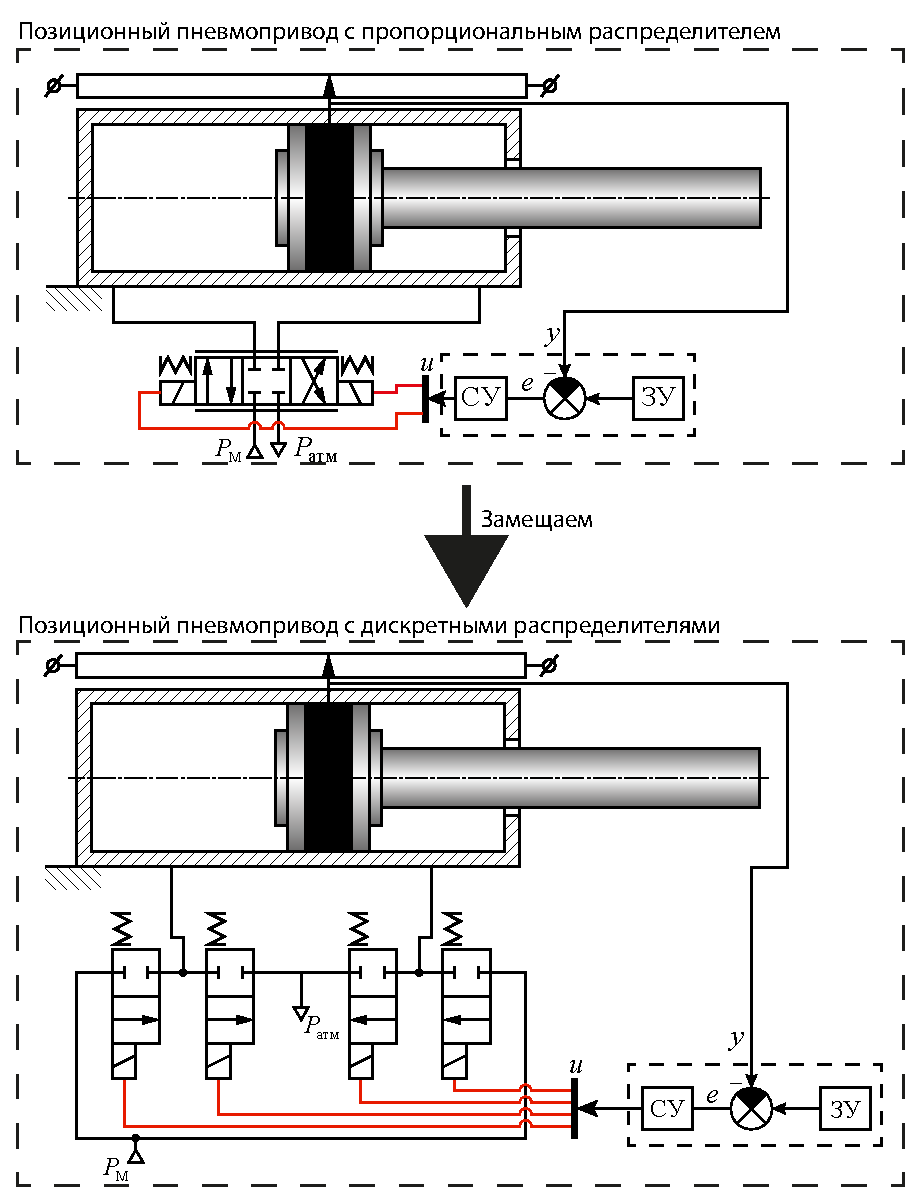
\includegraphics[width=\textwidth]{actuator_change.eps}
			\end{center}
		}

		\column{0.48\textwidth}
		\begin{block}{\scriptsize \textbf{Типовые области применнеия позиционного пневмопривода}}
			\centering
			\begin{itemize}
				\item \scriptsize \textbf{Энергетика} и коммунальное хозяйство
				\item \scriptsize Управление \textbf{запорной арматурой}
				\item \scriptsize Робототехника
				\item \scriptsize Станкостроение
				\item \scriptsize Промышленная автоматизация
				\item \scriptsize Пищевая и фармацевтическая промышленность
				\item \scriptsize И т.д.
			\end{itemize}
		\end{block}
	\end{columns}
\end{frame}

\begin{frame}
	\frametitle{Историческое развитие}
	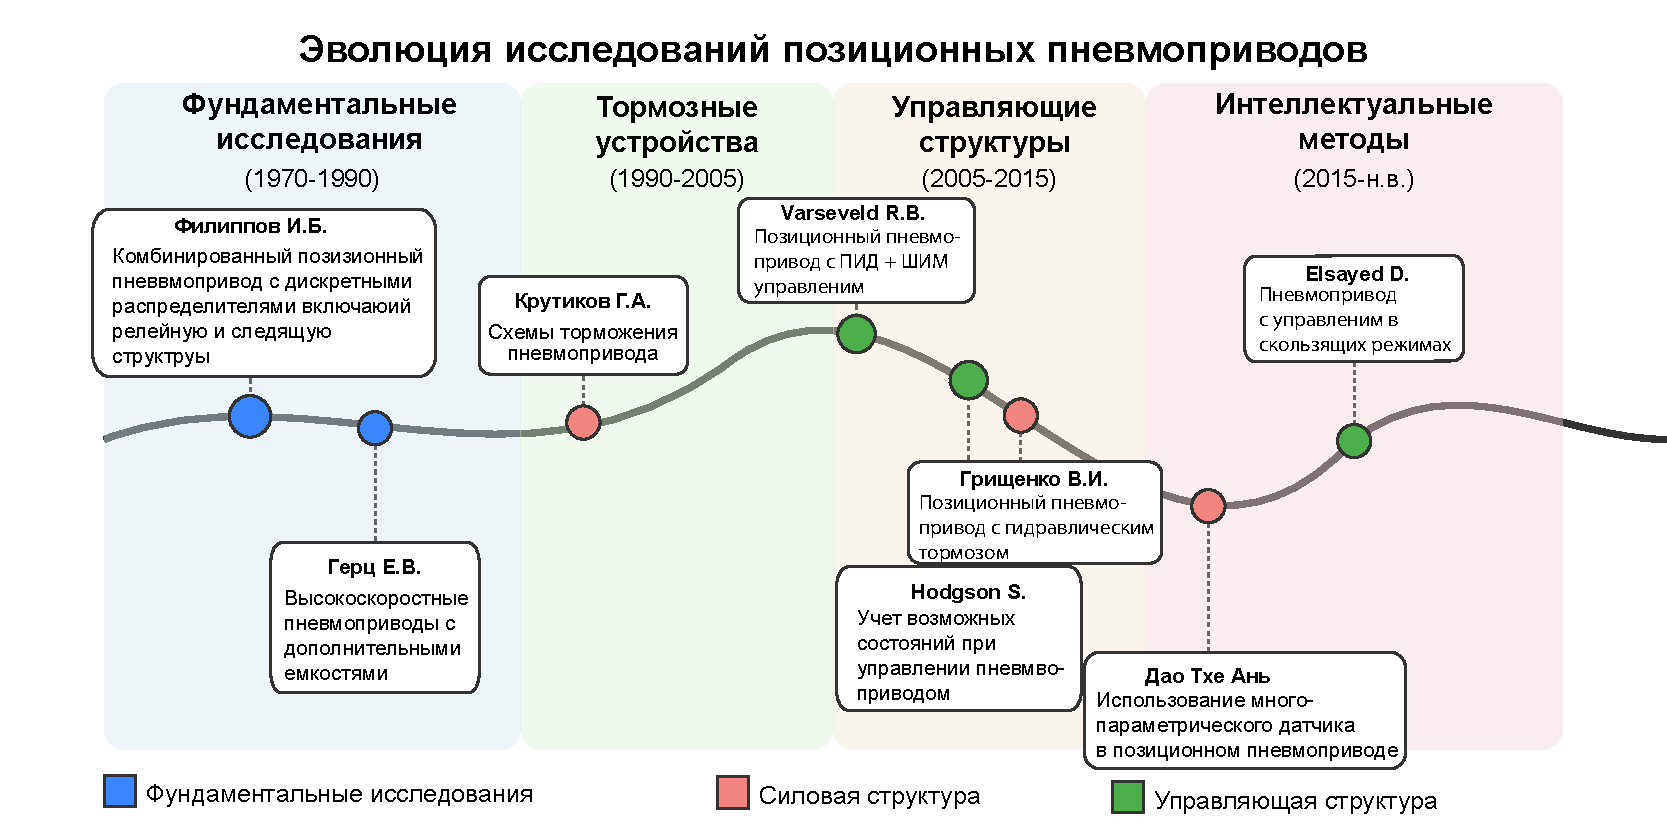
\includegraphics[width=\textwidth]{timeline-illustration.pdf}
	\begin{block}{Научное противоречие}
		\scriptsize Противоречие между улучшением статико-динамических характеристик позиционного пневмопривода с дискретными распределителями и сохранением качества рабочего процесса при неизученности их взаимовлияния
	\end{block}
\end{frame}

\begin{frame}
	\frametitle{Подходы к решению проблем в позиционном пневмоприводе}

	\begin{columns}[T]
		\begin{column}{0.48\textwidth}
			\textcolor{red}{ \scriptsize\textbf{Силовая структура позиционного пневмопривода}}

			\begin{itemize}\setlength{\itemsep}{0pt}
				\item \scriptsize Дополнительные тормозные устройства для повышения \textbf{точности}
				\item \scriptsize Применение дополнительных емкостей для повышения \textbf{быстродействия}
				\item \scriptsize Непосредственный выхлоп в атмосферу для повышения \textbf{быстродействия}
				\item \scriptsize Комбинированные позиционные пневмоприводы
			\end{itemize}

			\textcolor{green!50!black}{\scriptsize\textbf{Управляющая структура позиционного пневмопривода}}

			\begin{itemize}\setlength{\itemsep}{0pt}
				\item \scriptsize Управление в скользящих режимах c учетом \textbf{возможных состояний}
				\item \scriptsize Адаптивное ПИД с прогнозированием
				\item \scriptsize Прогнозное управление (MPC)
				\item \scriptsize Нечеткая логика
			\end{itemize}
		\end{column}

		\begin{column}{0.48\textwidth}
			\begin{block}{\scriptsize \textbf{Объект}}
				\scriptsize \textbf{Позиционный пневмопривод с дискретными распределителями}
				\begin{itemize}
					\item \scriptsize Пневмоцилиндр двустороннего действия
					\item \scriptsize Четыре дискретных распределителя
				\end{itemize}
			\end{block}

			\vspace{0.3cm}

			\begin{center}
				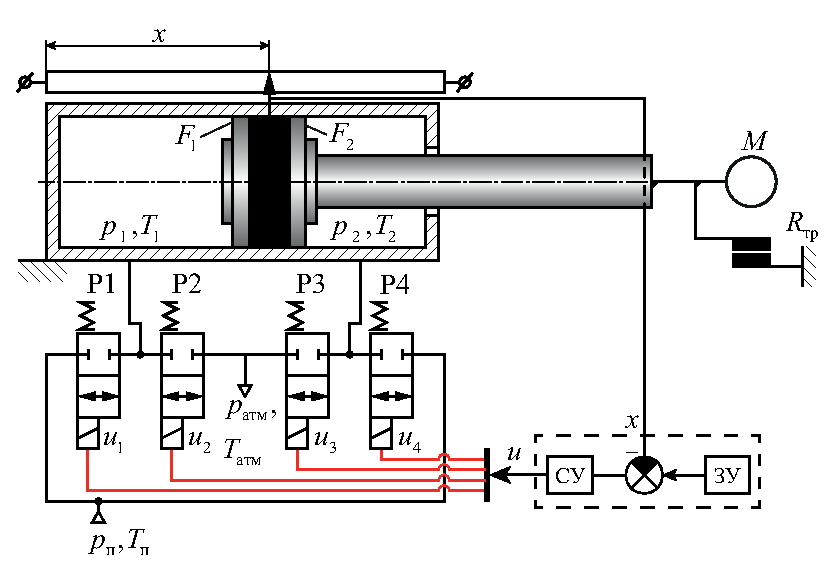
\includegraphics[width=\textwidth]{actuator_calc_schemne.eps}
			\end{center}
		\end{column}
	\end{columns}

	% \begin{columns}[T]
	% 	\begin{column}{0.48\textwidth}
	% 		\begin{center}
	% 			{\color{red}\footnotesize Возрастание себестоимости}
	% 		\end{center}
	% 	\end{column}

	% 	\begin{column}{0.48\textwidth}
	% 		\begin{center}
	% 			{\color{green!50!black}\footnotesize Сохранение экономичности и простоты}
	% 		\end{center}
	% 	\end{column}
	% \end{columns}

	% \vspace{0.3cm}
	% \begin{alertblock}{Вывод}
	% 	\centering \small
	% 	Конструкционные решения нивелируют ключевые преимущества \\
	% 	дискретных распределителей — экономичность и простоту
	% \end{alertblock}
\end{frame}

\begin{frame}
	\frametitle{Научная проблема и цель исследования}

	\begin{columns}
		\begin{column}{0.48\textwidth}
			\textbf{Научная проблема:}
			\begin{itemize}
				\item \scriptsize Отсутствуют исследования о влиянии улучшения статико-динамических
				      характеристик на качество рабочего процесса позиционного пневмопривода с дискретными
				      распределителями, приводящем к увеличению частоты срабатывания распределителей
			\end{itemize}

			\vspace{0.15cm}
			\begin{block}{\textbf{Цель}}
				\scriptsize Комплексное повышение статико-динамических и ресурсных показателей позиционного пневмопривода
				с дискретными распределителями в условиях их конфликтности без специальных дополнительных устройств
			\end{block}

			% \vspace{0.05cm}
			% \begin{alertblock}{\textbf{Ключевой тезис:}}
			% 	\scriptsize Необходимо исследовать компромисс между улучшением статико-динамических характеристик позиционного пневмопривода с дискретными распределителями и сохранением качества рабочего процесса для обеспечения оптимального баланса точности, быстродействия и надежности
			% \end{alertblock}
		\end{column}

		\begin{column}{0.48\textwidth}
			\centering
			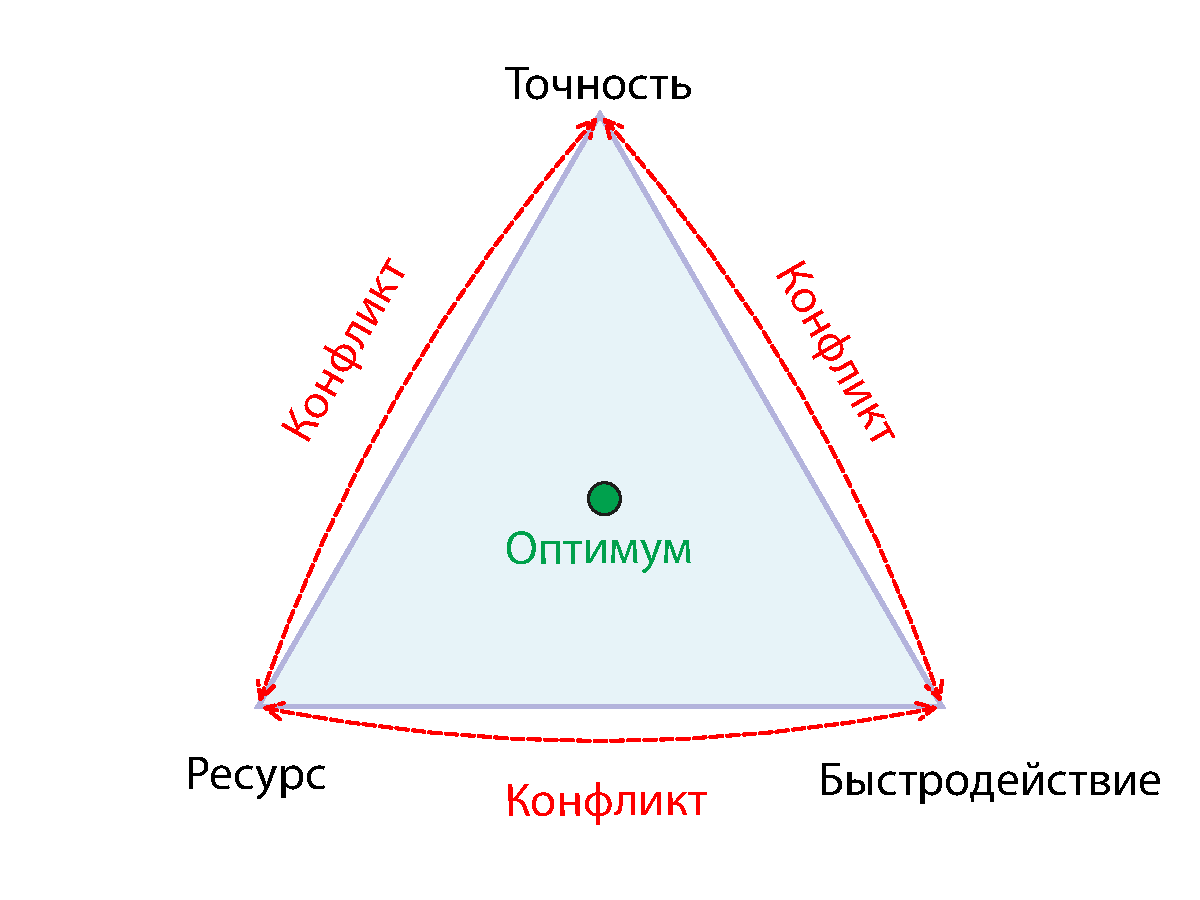
\includegraphics[width=1\textwidth]{conflict_triangle.pdf}
		\end{column}
	\end{columns}
\end{frame}

\begin{frame}
	\frametitle{Задачи исследования}
	\begin{enumerate}
	\item \scriptsize Разработать комплексную математическую модель пневмопривода с дискретными распределителями,
	      включающую силовую и управляющие структуры, учитывающую нелинейные эффекты
	      при функционировании и реализующую различные алгоритмы управления.

	\item \scriptsize Провести комплексный анализ различных структур пневмопривода для выявления оптимальных
	      режимов переключения при позиционировании рабочего органа.

	\item \scriptsize Провести натурный эксперимент для подтверждения работоспособности предлагаемых структур
	      и достоверности результатов, полученных по разработанной математической модели.

	\item \scriptsize Разработать методику многокритериального структурно-\allowbreak па\-ра\-ме\-три\-че\-ско\-го
	      синтеза, основанную на использовании фронтов Парето.

	\item \scriptsize Определить взаимосвязь между конфликтными статико-динамическими и ресурсными
	      показателями для позиционных пневмоприводов различной структуры на
	      основе анализа фронтов Парето, выявить области их предпочтительные применения.

	\item \scriptsize Сформировать практические рекомендации по выбору оптимальной структуры
	      позиционного пневмопривода с дискретными распределителями.

	\end{enumerate}
\end{frame}
